\documentclass[a4paper,12pt]{book}

\usepackage[polish]{babel}
\usepackage[utf8]{inputenc}
\usepackage[OT4]{fontenc}
\usepackage{tabularx}
\usepackage{geometry}
\usepackage[pdftex]{graphicx}
\usepackage[T1]{fontenc}
\usepackage{listings}
\usepackage{subfigure}

\geometry{verbose,a4paper,tmargin=2.5cm,bmargin=2.5cm,lmargin=3cm,rmargin=2.5cm}

\linespread{1.3}

\pagestyle{empty}

\author{Jakub Odias}
\title{Konstrukcja platformy sprzętowej dla potrzeb wbudowanego systemu Linux}

\begin{document}
	{\fontfamily{phv}\selectfont
	\begin{titlepage}
		\vspace*{15pt}
		\begin{figure}[htp]
			\begin{center}
				
\includegraphics[scale=0.25]{img/polsl.png}
			\end{center}
		\end{figure}

		\vspace{-10pt}
		\begin{center}
			
			\Large{\textbf{P}}\large{\textbf{OLITECHNIKA}}\Large{\textbf{ Ś}}\large{\textbf{LĄSKA}}\\

			\vspace{12pt}
			
			\Large{\textbf{W}}\large{\textbf{YDZIAŁ }}\Large{\textbf{A}}\large{\textbf{UTOMATYKI, }}\Large{\textbf{E}}\large{\textbf{LEKTRONIKI I }}\Large{\textbf{I}}\large{\textbf{NFORMATYKI}}\\

			\vspace{80pt}
			
			\Large{Praca dyplomowa magisterska}
			
			\vspace{40pt}
			
			\large{Konstrukcja platformy sprzętowej dla potrzeb \\wbudowanego systemu Linux}
		\end{center}
		\vspace{90pt}
		
		\begin{flushleft}
			\large{Autor: Jakub Odias}\\
			\vspace{5pt}
			\large{Kierujący pracą: dr inż. Krzysztof Tokarz}\\

			\vspace{110pt}
			\normalsize{Gliwice, sierpień 2009}
		\end{flushleft}
	\end{titlepage}}

	\tableofcontents

%------------------------------------------------------------------------------------
% WSTĘP
%------------------------------------------------------------------------------------

	\chapter{Wstęp}
		\section{Wprowadzenie}
			Wraz z rozwojem informatyki pojawia się coraz więcej układów sprzętowych, różnorodnych protokołów oraz użytecznych aplikacji i bibliotek. Aby napisać sterownik urządzenia lub programową obsługę dla danego protokołu, należy zazwyczaj poświęcić dużo czasu i zasobów na zapoznanie się z dokumentacją, napisanie programu oraz wystarczające przetestowanie.\\
			Dlatego podczas tworzenia zaawansowanego układu sprzętowego, wygodnym rozwiązaniem jest użycie gotowego i stabilnego kodu, który obsłuży większość potrzebnych użytkownikowi funkcjonalności. Firmy zajmujące się produkcją nowych urządzeń, np. telefonów komórkowych czy routerów bezprzewodowych, zazwyczaj wykorzystują rozwijane przez siebie aplikacje lub proste systemy operacyjne w celu przyspieszenia wstępnej fazy uruchamiania nowego oprogramowania oraz późniejszego efektywnego zarządzania zasobami. Możliwe jest także zastosowanie gotowych rozwiązań, takich jak zaawansowane systemy operacyjne Windows Embedded i Linux; wadą wbudowanej wersji Windowsa jest niestety to że nie jest to darmowe oprogramowanie, oraz w przeciwieństwie do Linuksa nie posiada ogólnodostępnego kodu źródłowego. Dzięki udostępnieniu plików źródłowych jądra systemu Linux na licencji GNU General Public License 2 \cite{gnu_gpl_v2}, każdy programista może dla swoich potrzeb napisać sterownik, a następnie udostępnić go innym - w ten sposób dodawanie nowych funkcjonalności oraz poprawianie ewentualnych błędów jest znacznie uproszczone.\\
			Dzięki wiedzy o tym w jaki sposób zaprojektować platformę sprzętową, umożliwiającą uruchomienie systemu operacyjnego na prostym układzie mikroprocesorowym, można stworzyć urządzenie które ma bardzo rozbudowane możliwości, porównywalne z tymi dostępnymi w urządzeniach przenośnych.
		\section{Cel pracy}
			Celem niniejszej pracy magisterskiej jest konstrukcja platformy sprzętowej dostosowanej do potrzeb wbudowanego systemu Linux (ang. Embedded Linux). Platforma ma mieć mozliwość podłączenia pamięci masowych typu Compact  Flash lub dysk IDE, wyświetlaczy graficznych LCD, urządzeń USB oraz sieci Ethernet.\\
			Głównym zadaniem było zaprojektowanie oraz wykonanie części sprzętowej projektu, spełniającej powyższe wymagania, a następnie zapoznanie się z wbudowaną wersją systemu Linux i jej implementacja na gotowym układzie.\\
		\section{Wbudowany Linux}
			W odróżnieniu od systemu operacyjnego Linux, stosowanego w komputerach domowych lub na serwerach, wbudowana wersja jest przeznaczona dla urządzeń z ograniczonymi zasobami, np. urządzeń mobilnych. Pełnią one ściśle określoną rolę, więc nie muszą zawierać zbędnego lub mało używanego oprogramowania oraz niepotrzebnych sterowników. Dodatkowo mają zazwyczaj ograniczoną ilość pamięci RAM, szybkość pracy procesora oraz niewiele zasobów dyskowych więc ważna jest także odpowiednia konfiguracja i optymalizacja takiego systemu.\\
			Określenie 'Wbudowany Linux' oznacza zatem jedynie konfigurację systemu dla konkretnych potrzeb - jądro Linuksa jest niemal identyczne jak w przypadku komputerów klasy PC lub podobnych.
		\section{Platforma sprzętowa}
			Podczas konstruowania uniwersalnej platformy sprzętowej dla Linuksa istotne jest wzięcie pod uwagę następujących czynników:
			\begin{itemize}
				\item Linux jest systemem 32-bitowym więc procesor użyty w projekcie również powinien mieć architekturę 32-bitową. Co prawda istnieją wersje Linuksa dostosowane dla mikroprocesorów 8- lub 16-bitowych, jednak nie są one dostatecznie wspierane.
				\item System operacyjny Linux wymaga żeby procesor implementował jednostkę zarządzania pamięcią (MMU) w celu efektywnego i bezpiecznego używania pamięci. Istnieje okrojona wersja $\mu$cLinux\cite{uclinux} dostosowana do potrzeb mikroprocesorów niewyposażonych w MMU.
				\item Tworzony układ powinien móc wykonać dostateczną liczbę operacji na sekundę oraz mieć ilość pamięci RAM wystarczającą do uruchomienia zaawansowanego systemu operacyjnego.
				\item Platforma powinna umożliwić podłączenie jak najmniejszym kosztem sieci Ethernet, urządzeń USB oraz wszelkich innych układów.
			\end{itemize}
		\section{Przykładowe implementacje}
			Linux jest obecnie najpopularniejszym systemem operacyjnym wśród producentów systemów wbudowanych m.in. telefonów komórkowych, Palmtopów, przełączników i routerów sieciowych oraz systemów przemysłowych.\\
			Podczas projektowania układu pomocne jest wzorowanie się na działających rozwiązaniach, które pełnią podobne funkcje.\\
			W dodatku \ref{app:przykladowe_projekty} znajduje się lista stron WWW mieszczących projekty, z których korzystał autor tej pracy.



%------------------------------------------------------------------------------------
% CZĘŚĆ SPRZĘTOWA
%------------------------------------------------------------------------------------

	\chapter{Część sprzętowa}
		\section{Wprowadzenie}
			W tej części zostanie przedstawiony dobór, wraz z objaśnieniem, wszystkich układów sprzętowych użytych w projekcie oraz opis zagadnień na które należało zwracać uwagę podczas projektowania platformy.\\
			W dodatku \ref{app:gotowy_projekt} znajdują się schematy i zdjęcia zaprojektowanego układu.
		\section{Mikroprocesor}
			\subsection{Wymagania}
				Podczas wyboru mikroprocesora, który będzie stanowił rdzeń platformy, kierowano się tym aby wybrany układ scalony posiadał następujące cechy:
				\begin{itemize}
					\item architektura 32-bitowa
					\item jednostka zarządzania pamięcią MMU
					\item maksymalna szybkość pracy mikroprocesora wystarczająca do efektywnego działania systemu operacyjnego
					\item sprzętowa obsługa portów USB i Ethernet
					\item interfejs SPI i/lub MMC w celu podłączenia kart pamięci SD/MMC
					\item wbudowany kontroler pamięci SDRAM
					\item dostępność układu w obudowie umożliwiającej stosunkowo łatwe przylutowanie np. TQFP
				\end{itemize}
			\subsection{Porównanie dostępnych układów}
				Na rynku jest dostępnych wiele procesorów o architekturach spełniających wymagania projektu m.in. x86, PowerPC, MIPS, ARM i AVR32, jednak jedynie 2 ostatnie z nich są łatwo dostępne w ilościach detalicznych.\\
				Zarówno ARM jak i AVR32 są wspierane przez jądro systemu Linux, jednak kod dla 32-bitowej architektury mikrokontrolerów AVR został udostępniony stosunkowo niedawno, bo dopiero w wersji 2.6.19. W związku z tym zdecydowano się na wykorzystanie jednego z procesorów zawierających rdzeń firmy ARM\cite{arm}, które już od dłuższego czasu posiadają stabilne sterowniki w źródłach kernela.\\
				Układy oparte o rdzenie ARM są produkowane przez różne firmy np. Philips zajmuje się wytwarzaniem mikrokontrolerów ARM7TDMI, niestety nie są one wyposażone w jednostkę MMU, natomiast firma Atmel jest uznanym producentem układów m.in. z rodzin ARM9TDMI i ARM9E. Mikroprocesory z nowszymi rdzeniami, takimi jak XScale i Cortex, są trudno dostępne do zakupu oraz występują zazwyczaj w obudowach BGA.\\
				Po zapoznaniu z ofertą firmy Atmel, okazało się że jedynie mikrokontrolery AT91RM9200 i AT91SAM9260 spełniają wymagania projektu (są dostępne w Polsce oraz występują w obudowach QFP208). W tabeli \ref{tab:arm_comparison} znajduje się porównanie najważniejszych cech obu układów.
				
				\begin{table}[]
					%\extrarowheight=3pt
					\begin{tabularx}{\textwidth }{|c|X|X|}
						\hline \textbf{Cecha} &\textbf{AT91RM9200} & \textbf{AT91SAM9260} \\ 
						\hline Rdzeń & ARM920T & ARM926EJ-S - rozszerzone rozkazy DSP, technologia ARM Jazelle\textsuperscript{\textregistered} dla Javy \\
						\hline Szybkość & 200 MIPS @ 180 MHz & 200 MIPS @ 180 MHz \\
							procesora & & \\
						\hline Pamięć cache & 16kB dane, 16kB instrukcje & 8kB dane i 8kB instrukcje \\
						\hline Wbudowana pamięć & 16kB SRAM, 128kB ROM & 4kB SRAM, 32 kB ROM \\
						\hline Ethernet & kontroler MAC 10/100T z interfejsem MII & kontroler MAC 10/100T z interfejsem MII \\
						\hline USB & USB 2.0 - tryb urządzenia i gospodarza & USB 2.0 - tryb urządzenia i gospodarza \\
						\hline Możliwość podłączenia & SDRAM, pamięć statyczna, Dataflash & SDRAM, pamięć statyczna, Dataflash \\
							zewn. pamięci & & \\
						\hline Interfejs MMC & tak & tak \\
						\hline Debug Unit & tak & tak \\
						\hline JTAG & tak & tak \\
						\hline SPI & tak, możliwość podłączenia 4 układów & tak, możliwość podłączenia 4 układów \\
						\hline TWI & tak & tak - multimaster \\
						\hline SSC & tak - 3 interfejsy & tak - 1 interfejs \\
						\hline Liczba linii PIO & 94 & 96 \\
						\hline Dodatkowe cechy & - & interfejs do rozpoznawania obrazów, kontroler resetu, 4 zapasowe rejestry\\
						\hline 
					\end{tabularx}
					\caption{Porównanie mikroprocesorów AT91RM9200 i AT91SAM9260}
					\label{tab:arm_comparison}
				\end{table}
			Pomimo tego że mikrokontroler AT91SAM9260 posiada nowszy rdzeń i więcej wbudowanych układów sprzętowych niż AT91RM9200, zdecydowano się na wykorzystanie drugiego z nich z następujących przyczyn:
			\begin{itemize}
				\item Pamięć SRAM musi pomieścić program ładujący (ang. bootloader) - limit 4kB w przypadku nowszego układu mógłby spowodować problemy przy implementacji wszystkich potrzebnych funkcji.
				\item Kilka układów wewnętrznych, m.in. interfejs Ethernet, SPI i MMC, dzieli między sobą te same nóżki mikrokontrolera AT91SAM9260 co wymaga multipleksowania programowego i sprzętowego.
				\item Na procesorze AT91RM9200 zostały oparte projekty przedstawione w dodatku \ref{app:przykladowe_projekty} - w ich źródłach znajdują się poprawione sterowniki urządzeń.
			\end{itemize}
		\section{Nośniki pamięci}
			\subsection{Pamięć SDRAM}			
				W projekcie wykorzystano 2 popularne i tanie układy K4S561632J firmy Samsung - każdy z nich posiada pojemność 16777216 słów 16-bitowych, co po równoległym połączeniu w jedną magistralę 32-bitową daje pojemność 64MB. \\
				Wybrany mikrokontroler posiada zarówno interfejs do obsługi zewnętrznej magistrali (linie A0-A25 i D0-D31) jak i kontroler SDRAM, który odpowiada m.in. za odświeżanie komórek pamięci.\\
				Pamięć synchroniczna jest wykorzystywana jako pamięć operacyjna platformy - program rozruchowy inicjalizuje ją, a następnie ładuje do niej jądro systemu Linux i przekazuje mu kontrolę.
				
			\subsection{Pamięć NAND i NOR Flash}
				W urządzeniach mobilnych popularne jest zastosowanie układów pamięci NAND lub NOR Flash, jednak w omawianym projekcie nie zostały one użyte z powodu ich wysokiej ceny. Ponieważ pamięć tego typu jest bardzo szybka, ale posiada ograniczoną liczbę zapisów, dobrym pomysłem jest jej wykorzystanie do przechowywania programu rozruchowego oraz jądra systemu Linux.
				
			\subsection{Pamięć Serial Dataflash}
				Pamięć Serial Dataflash firmy Atmel (dowolny model z serii AT45DB) jest tanią alternatywą dla układów NAND i NOR Flash. Zgodnie ze specyfikacją, szeregowy interfejs pozwala na osiągnięcie częstotliwości taktowania równej 66MHz.\\
				Wykorzystany układ scalony AT45DB041D posiada 512kB pamięci i jego zadaniem jest przechowywanie bootloadera odpowiedzialnego za inicjalizację większości układów i załadowanie kernela z karty pamięci SD/MMC.\\
				Mikrokontroler AT91RM9200 po zresetowaniu szuka programu w pamięci Serial Dataflash podłączonej do interfejsu SPI0. Jeśli zostanie znaleziony prawidłowy program, zostanie on załadowany do pamięci SRAM i stamtąd uruchomiony.
			\subsection{Karty pamięci}
				Platforma ma możliwość włożenia 2 kart pamięci SD/MMC. Na pierwszej z nich znajduje się główny system plików i korzysta ona ze standardowego równoległego, 4-bitowego interfejsu MCI (Multimedia Card Interface) w celu jak najszybszej pracy. Druga z kart używa szeregowego interfejsu SPI i może służyć do zapisywania danych wykorzystywanych przez użytkownika.
		\section{Standard sieciowy Ethernet}
		\section{Standard transmisji USB}
			USB (Universal Serial Bus) jest bardzo popularnym standardem szeregowej transmisji danych. Za jego pomocą można połączyć rozmaite urządzenia m.in. myszki, klawiatury, nośniki danych, kamery internetowe.
			\subsection{Host USB}
				Używany mikrokontroler posiada wbudowany kontroler USB w wersji 2.0, co umożliwia podłączanie urządzeń i transfer danych z prędkością do 12Mb/s.\\
				System Linux posiada wsparcie dla protokołu USB, zatem użytkownik nie musi zajmować się pisaniem skomplikowanego sterownika.
			\subsection{Urządzenie USB}
				Mikroprocesor AT91RM9200 może pełnić rolę urządzenia USB poprzez użycie pinów DDM i DDP. Możliwe jest wtedy podłączenie np. do komputera klasy PC, który działa w trybie hosta. Niestety, z powodu braku wystarczającej ilości miejsca na płytce drukowanej, tryb urządzenia USB nie jest dostępny w projekcie.\\
			Przykładowy schemat podłączenia, wraz z wartościami elementów, jest przedstawiony w rozwiązaniach zawartych w dodatku \ref{app:przykladowe_projekty}.
			
		\section{Wyświetlacz LCD}
			Jednym z założeniem projektu była możliwość podłączenia wyświetlacza LCD. Żeby móc wyświetlać chociażby konsolę systemu Linux ważne było zastosowanie układu o jak największej rozdzielczości.\\
			Zdecydowano się na wybór panelu TFT LQ043T3DX02 firmy Sharp - został on zastosowany w konsoli do gier Sony Playstation Portable\textsuperscript{\textregistered} i umożliwia wyświetlanie obrazu w 24-bitowej głębi koloru i rozdzielczości 480*272 pikseli.\\
			Aby odciążyć procesor od potrzeby odświeżania obrazu istotne jest zastosowanie specjalizowanego kontrolera wyświetlacza LCD.
			\subsection{Kontroler wyświetlacza}
				Większość dostępnych sterowników kolorowych paneli TFT nie jest w stanie obsłużyć wyświetlacza o dużej rozdzielczości w pełnej głębi koloru. Istotnym parametrem takiego układu jest ilość wbudowanej pamięci stosowanej do przechowywania wyświetlanego obrazu.\\
				W projekcie użyto sterownika SSD1906 firmy Solomon, który posiada 256kB pamięci SRAM i potrafi wyświetlać obraz w głębi 18 bitów. Dostępna pamięć układu pozwala jednak jedynie na wyświetlenie obrazu o rozdzielczości 480*272 pikseli używając 16 bitowej palety kolorów (480 * 272 * 16 bitów = 261120 bitów = 255 kB). Dodatkowo układ scalony SSD1906 posiada funkcje takie jak obracanie wyświetlanego obrazu, wybór okna wyświetlania i sterowanie podświetleniem poprzez specjalne linie.
		\section{Urządzenia peryferyjne mikrokontrolera}
			Układ scalony AT91RM9200 posiada wiele wbudowanych układów mogących pełnić różne funkcje. Poniżej znajduje się ich lista wraz z przykładowymi zastosowaniami.
			\begin{itemize}
				\item SPI
			\end{itemize}
		\section{Pozostałe układy}
			\subsection{JTAG}
				\label{sec:jtag}
			\subsection{Przetwornik Audio}
			\subsection{Inne możliwości}
		\section{Projekt platformy}
			\label{sec:projekt_platformy}
			\subsection{Główna płytka sprzętowa}
			\subsection{Dodatkowa płytka sprzętowa}
			\subsection{Programator}
				\label{sec:programator}
				Aby zaoszczędzić miejsce na głównej płytce wchodzącej w skład projektu, zdecydowałem że układy scalone, złącza, oraz pozostałe elementy używane tylko podczas programowania lub debuggowania układu będą znajdować się na osobnej płytce drukowanej dołączanej za pomocą przewodu do transmisji danych. TODO: photo itp
			\subsection{Lutowanie}
			\subsection{Gotowy układ}
				

			\subsection{Problemy}





%------------------------------------------------------------------------------------
% CZĘŚĆ PROGRAMOWA
%------------------------------------------------------------------------------------

	\chapter{Częć programowa}
		\section{Wprowadzenie}
		\section{Programowanie układu}
		
			\subsection{OpenOCD}
				Aby połączyć się z układem mikroprocesorowym za pomocą złącza JTAG należy zastosować specjalne oprogramowanie, które pozwoli na przetworzenie poleceń użytkownika, wydawanych za pośrednictwem komputera PC, na odpowiednie polecenia protokołu JTAG.\\
				Jedną z takich aplikacji jest Open On-Chip Debugger\cite{openocd}, który działa na zasadzie serwera uruchamianego w tle i oczekującego na polecenia użytkownika.
				\subsubsection{Instalacja}
					Stabilną wersję OpenOCD można pobrać ze strony domowej projektu, jednak wersja 0.2.0 nie współdziałała poprawnie z zastosowanym w tej pracy układem sprzętowym JTAG. W związku z tym użyto działającej wersji numer 1679 dostępnej pod kontrolą źródeł SVN na stronie twórców.\\
					Aby skompilować i zainstalować aplikację należy doinstalować sterowniki odpowiednie dla obsługi sprzętowej używanego programatora JTAG. Na systemie operacyjnym Debian wystarczy, mając uprawnienia administratora, wydać komendę:\\
					\texttt{apt-get install libftdi1 libftdi-dev libusb-dev}\\
					W celu ściągnięcia i zainstalowania samej aplikacji należy wykonać ciąg następujących poleceń:\\
					\texttt{svn checkout -r 1679 svn://svn.berlios.de/openocd/trunk} - spowoduje pobranie z SVN-a odpowiedniej wersji OpenOCD\\
					\texttt{./bootstrap} - wstępna konfiguracja\\
					\texttt{./configure --enable-maintainer-mode --enable-ft2232\_libftdi --prefix=/usr} - konfiguracja aplikacji; dołączenie biblioteki LibFTDI i ustawienie katalogu gdzie ma zostać zainstalowana na /usr\\
					\texttt{make \&\& make install} - kompilacja i instalacja\\
					Po poprawnym wykonaniu powyższych komend powinniśmy móc uruchomić oprogramowanie poprzez wykonanie polecenia \texttt{openocd}
					
				\subsubsection{Konfiguracja}
					Możliwe jest podanie opcji konfiguracyjnych bezpośrednio przy uruchomieniu OpenOCD lub zastosowanie plików konfiguracyjnych. Zgodnie z zaleceniami twórców, istotny jest podział konfiguracji na części istotne dla zastosowanego interfejsu służącego do programowania, używanego procesora oraz ustawień dodatkowych układów np. zewnętrznej pamięci SDRAM używanej w projekcie. W związku z tym ustawienia zostały podzielone na 4 części:
					\begin{itemize}
						\item{\texttt{openocd.cfg}}\\
							Główny plik konfiguracyjny definiujący m.in. używane porty.
							\begin{lstlisting}[basicstyle={\footnotesize\ttfamily}]
# Main configuration file
telnet_port 4444
gdb_port 3333
gdb_memory_map enable
gdb_flash_program enable
init
reset halt
							\end{lstlisting}
						\item{\texttt{interface/turtelizer.cfg}}\\
							Ustawienia interfejsu sprzętowego służącego do programowania.\\
							Opcja \texttt{jtag\_khz} służy do ustawiania szybkości interfejsu, lecz powinna być zmieniana dopiero po ustawieniu odpowiedniej szybkości pracy mikroprocesora.
							\begin{lstlisting}[basicstyle={\footnotesize\ttfamily}]
# Configuration file for programming interface
interface ft2232
ft2232_device_desc "Turtelizer JTAG/RS232 Adapter"
ft2232_layout turtelizer2
ft2232_vid_pid 0x0403 0xbdc8			
jtag_khz 8
jtag_nsrst_delay 200
jtag_ntrst_delay 200
							\end{lstlisting}
						\item{\texttt{target/at91rm9200.cfg}}\\
							Opcje specyficzne dla zastosowanego mikroprocesora.
							\begin{lstlisting}[basicstyle={\footnotesize\ttfamily}]
# Configuration file for AT91RM9200 microprocessor
reset_config srst_only srst_pulls_trst

if { [info exists CHIPNAME] } {
   set  _CHIPNAME $CHIPNAME
} else {
   set  _CHIPNAME at91rm9200
}
if { [info exists ENDIAN] } {
   set  _ENDIAN $ENDIAN
} else {
   set  _ENDIAN little
}
if { [info exists CPUTAPID ] } {
   set _CPUTAPID $CPUTAPID
} else {
   set _CPUTAPID 0x05b0203f
}
# Never allow the following!
if { $_CPUTAPID == 0x15b0203f } {
   puts "-------------------------------------------------"
   puts "- ERR: TapID 0x15b0203f is wrong for at91rm9200 -"
   puts "- ERR: The board has a JTAG select jumper       -"
   puts "-------------------------------------------------"
}

jtag newtap $_CHIPNAME cpu -irlen 4 -ircapture 0x1 -irmask 0xf 
   -expected-id $_CPUTAPID

# Create the GDB Target.
set _TARGETNAME [format "%s.cpu" $_CHIPNAME]
target create $_TARGETNAME arm920t -endian $_ENDIAN -chain-position 
   $_TARGETNAME 
# AT91RM9200 has a 16K block of sram @ 0x0020.0000
$_TARGETNAME configure -work-area-virt 0x00200000 -work-area-phys 
   0x00200000 -work-area-size 0x4000 -work-area-backup 1
							\end{lstlisting}
						\item{\texttt{board/at91rm9200\_lab.cfg}}\\
							Dodatkowy plik który może zawierać komendy używane do ustawienia szybkości pracy mikroprocesora, konfiguracji odpowiednich układów wewnętrznych, pamięci SDRAM itp.
					\end{itemize}
				\subsubsection{Uruchamianie}
					W celu uruchomienia demona OpenOCD należy wywołać poniższą komendę, podając nazwy używanych plików konfiguracyjnych:\\
					\texttt{openocd -f openocd.cfg -f interface/turtelizer.cfg -f target/at91rm9200.cfg}\\
					Możliwe jest wtedy podłączenie się np. przez program telnet na odpowiedni port (\texttt{telnet localhost 4444}) i wykonanie przykładowych poleceń:
					\begin{itemize}
						\item\texttt{mdb <address>} - przeczytaj bajt spod podanego adresu
						\item\texttt{mwb <address> <value>} - zapisz bajt pod podany adres
						\item\texttt{reset} - resetuje mikroprocesor
						\item\texttt{halt} - zatrzymuje pracę mikroprocesora
						\item\texttt{resume} - wznawia pracę mikroprocesora
						\item\texttt{reg} - wyświetla lub ustawia zawartość rejestru, np. \texttt{reg pc 0} zeruje licznik rozkazów
						\item\texttt{bp <address> <length>} - ustawia breakpoint pod podanym adresem, <length> to długość rozkazu obsługiwana przez mikroprocesor
						\item\texttt{load\_image <file> <adress>} - załadowanie pliku binarnego pod wskazany adres
						\item\texttt{arm920t cache\_info} - informacja o pamięci Cache zastosowanej w rdzeniu ARM920T
						\item\texttt{help} - pełny spis poleceń
					\end{itemize}
				
				
				
			\subsection{Debug Unit}
				s
			\subsection{Kompilator}
				k
			\subsection{GDB}
			\subsection{Eclipse}
		\section{Bootloader}
			\subsection{Bootloader inicjalizujący}
			\subsection{Bootloader główny}
		\section{Jądro Linuksa}
			\label{sec:linux_kernel}
			\subsection{Kompilacja}
			\subsection{Wybór modułów}
		\section{Dystrybucja Linuksa}
			\subsection{Buildroot}
		\section{System plików}
		\section{Moduły}
			\label{sec:linux_modules}
			\subsection{Ethernet}
			\subsection{Kontroler LCD}
		\section{Aplikacja demonstracyjna}
		
	\chapter{Podsumowanie}

	\bibliographystyle{plain}
	\bibliography{bibliography}
	
	
	
	\appendix
	
	\chapter{Gotowy projekt}
	\label{app:gotowy_projekt}
%		\begin{figure}[h]
%			\begin{center}
%				\label{fig:cpu_sch}
%				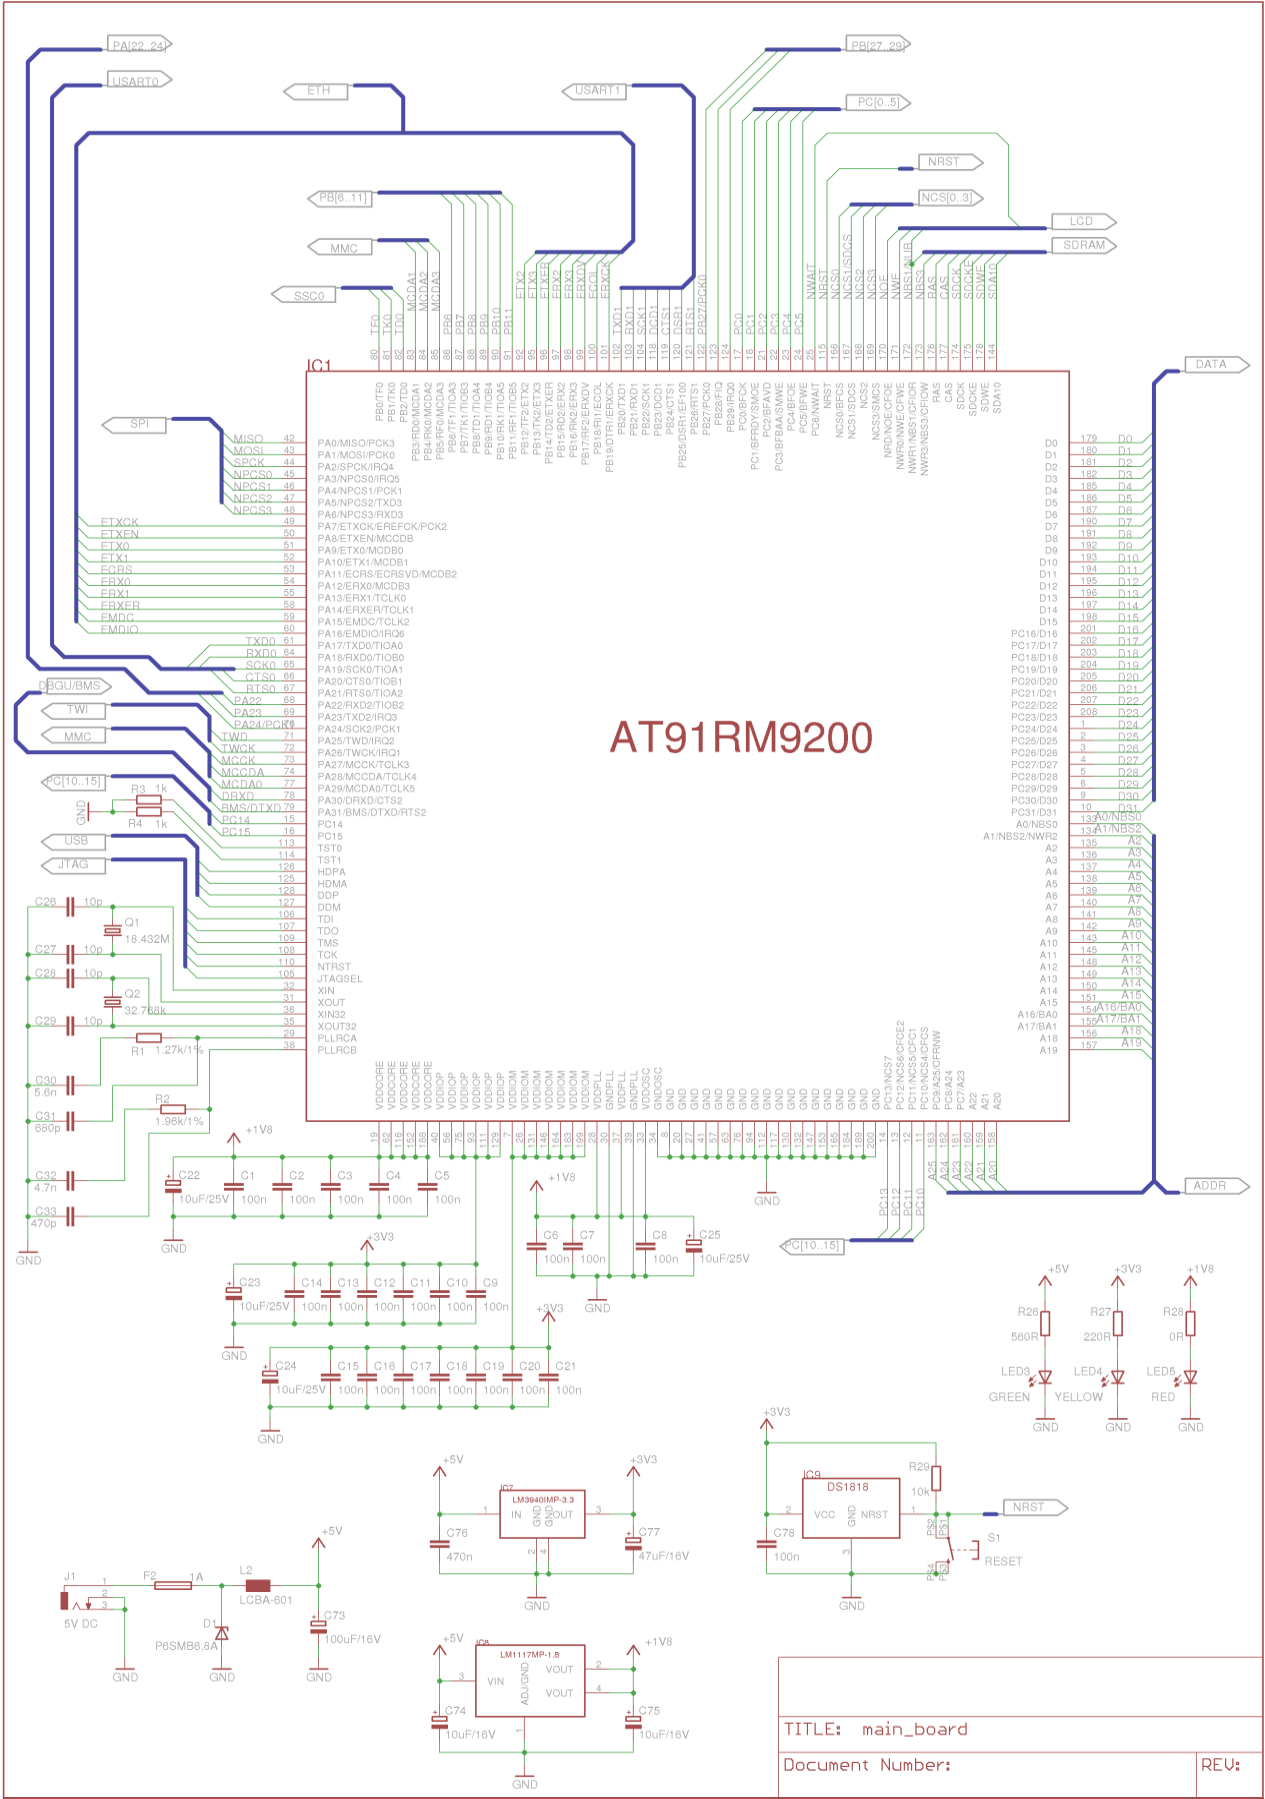
\includegraphics[scale=1.0]{img/cpu_sch.png}
%				\caption{Schemat podłączenia mikrokontrolera}
%			\end{center}
%		\end{figure}
%		
%		\begin{figure}[h]
%			\begin{center}
%				\label{fig:main_sch}
%				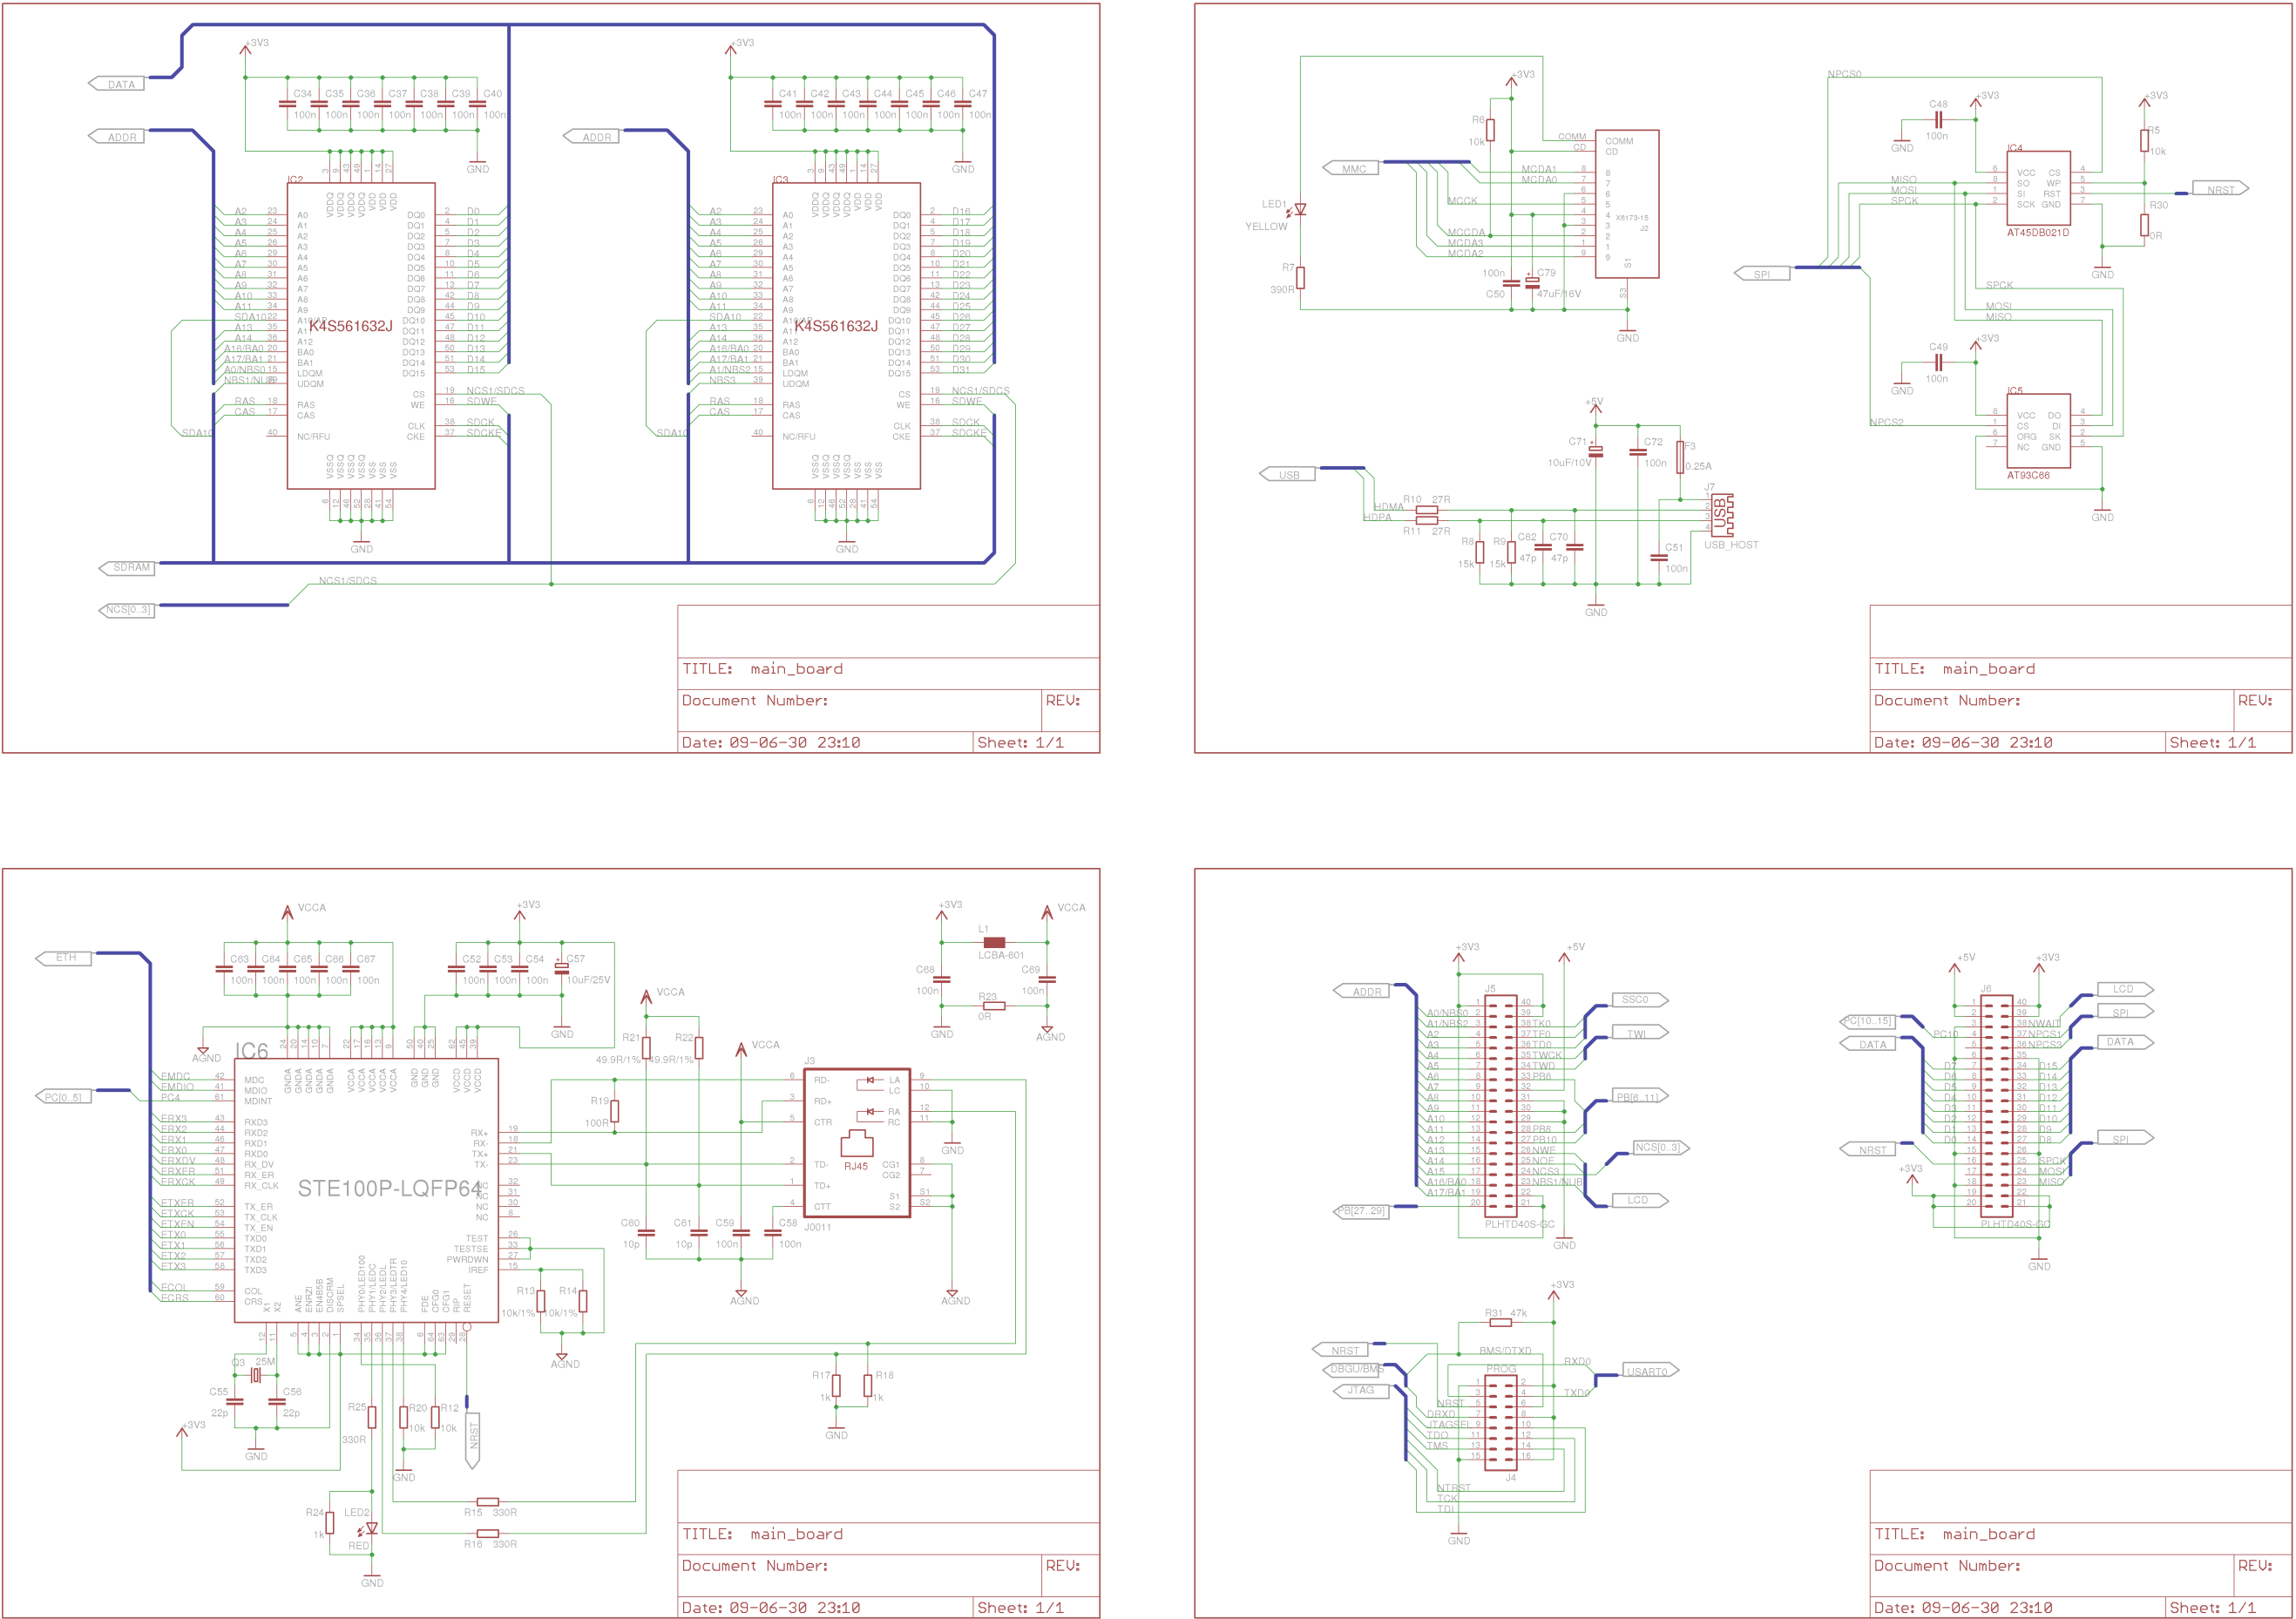
\includegraphics[scale=1.0,angle=90]{img/main_sch.png}
%				\caption{Schemat podłączenia dodatkowych układów do głównej części projektu}
%			\end{center}
%		\end{figure}
%		
%		\begin{figure}[]
%			\begin{center}
%				\label{fig:main_brd}
%				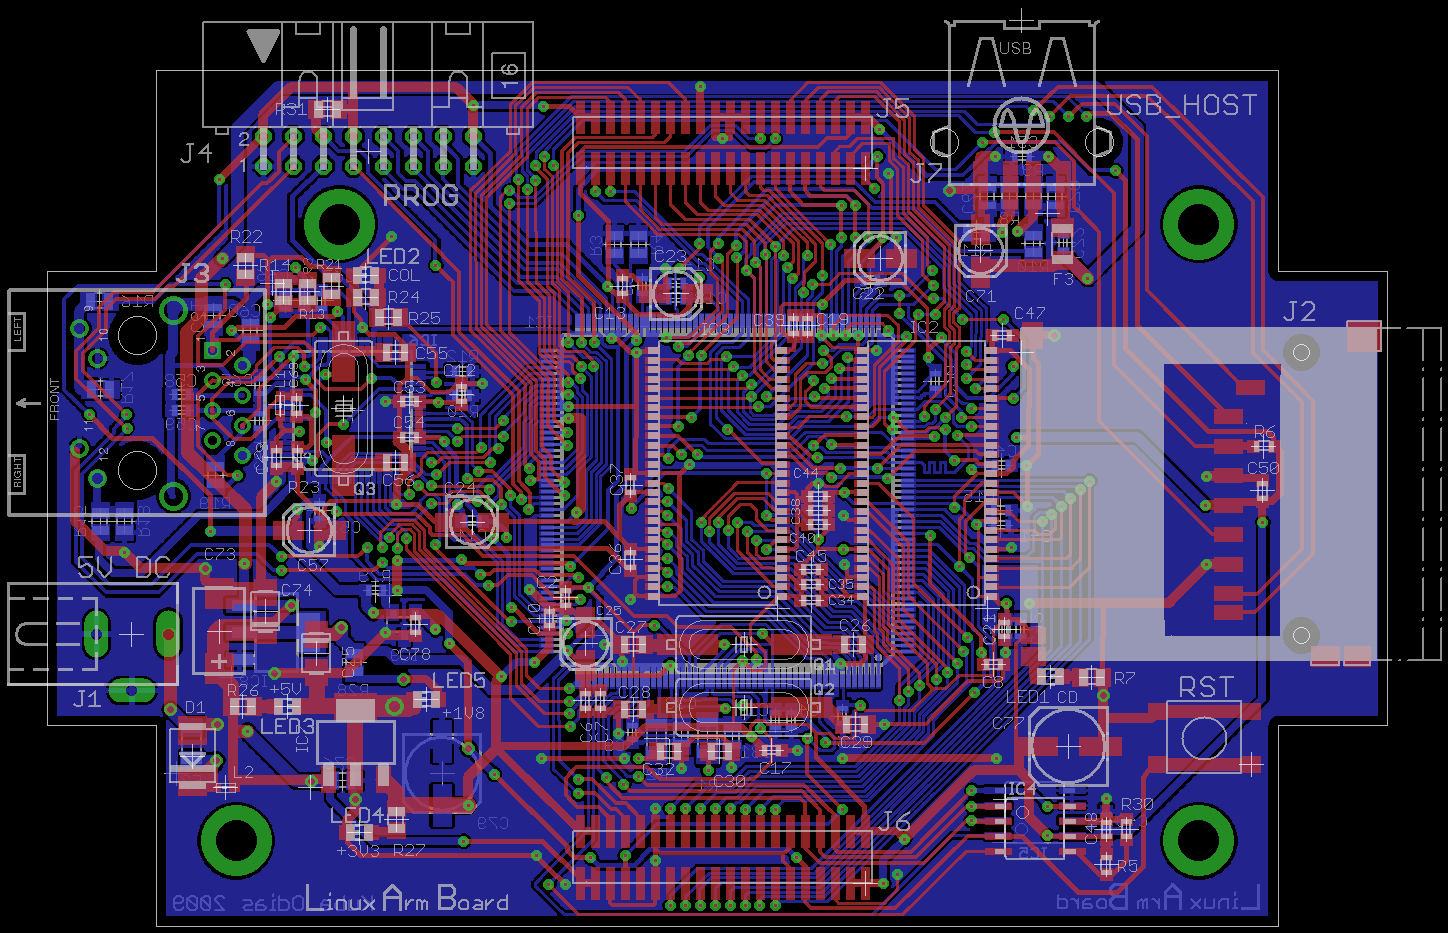
\includegraphics[scale=1.25]{img/main_brd.png}
%				\caption{Plik .brd programu Eagle dla głównej płytki}
%			\end{center}
%		\end{figure}
%		
%		\begin{figure}[]
%			\begin{center}
%				\label{fig:ext_brd}
%				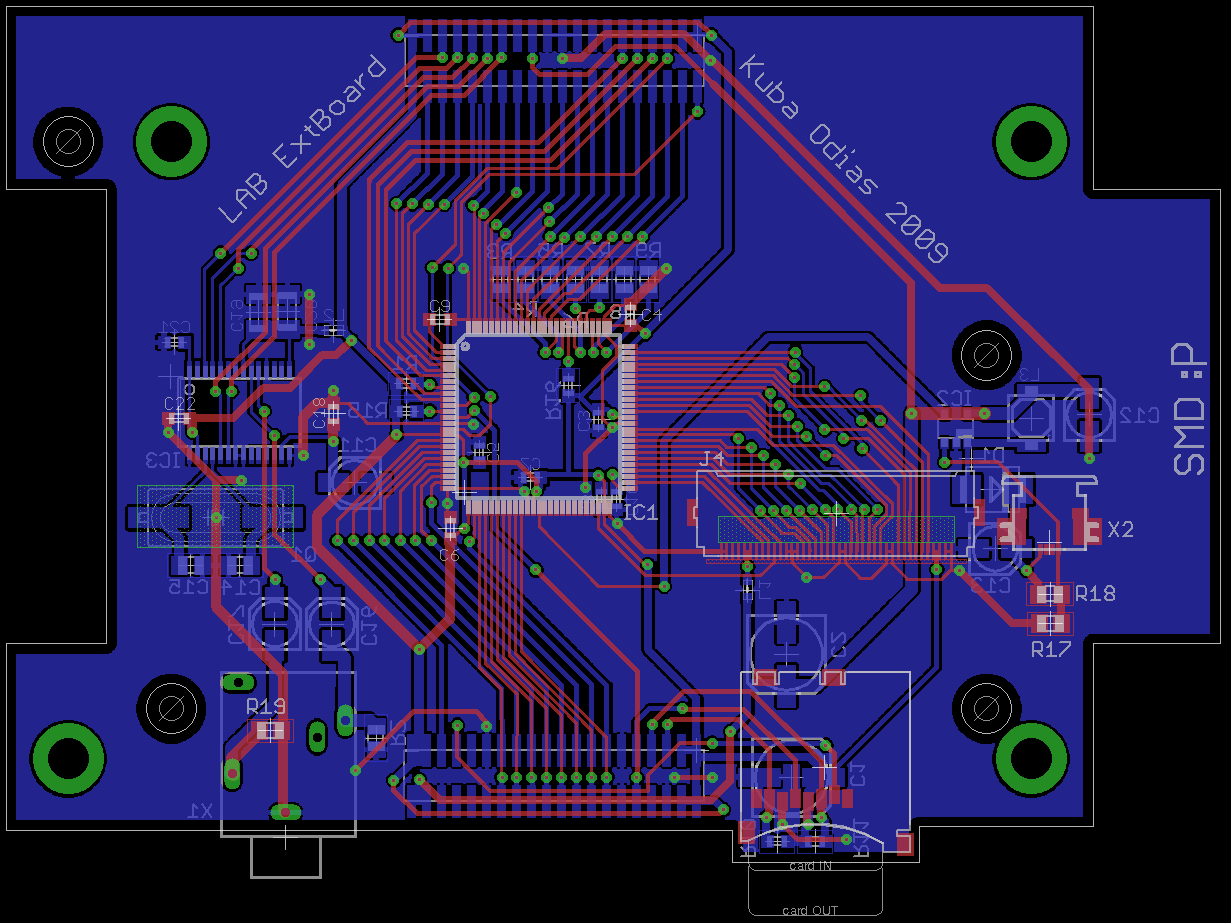
\includegraphics[scale=1.25]{img/ext_brd.png}
%				\caption{Plik .brd programu Eagle dla dodatkowej płytki}
%			\end{center}
%		\end{figure}
%		
%		\begin{figure}[]
%			\begin{center}
%				\subfigure[Górna strona]{\label{fig:pcb1-top}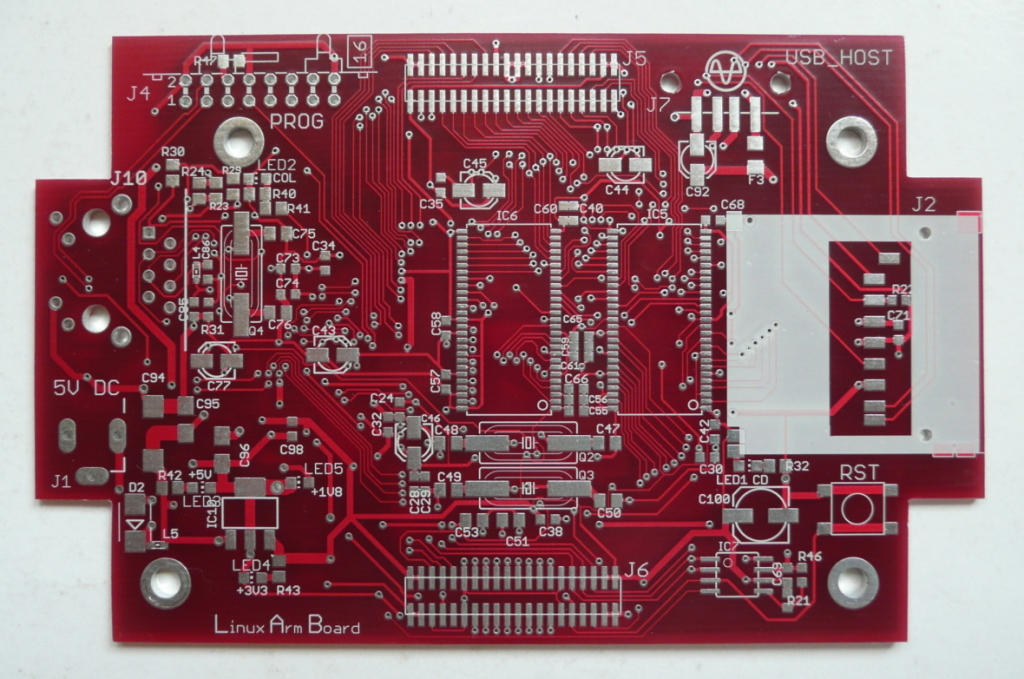
\includegraphics[scale=0.25,angle=90]{img/pcb1_top.jpg}}
%				\hspace{20pt}
%				\subfigure[Dolna strona]{\label{fig:pcb1-bottom}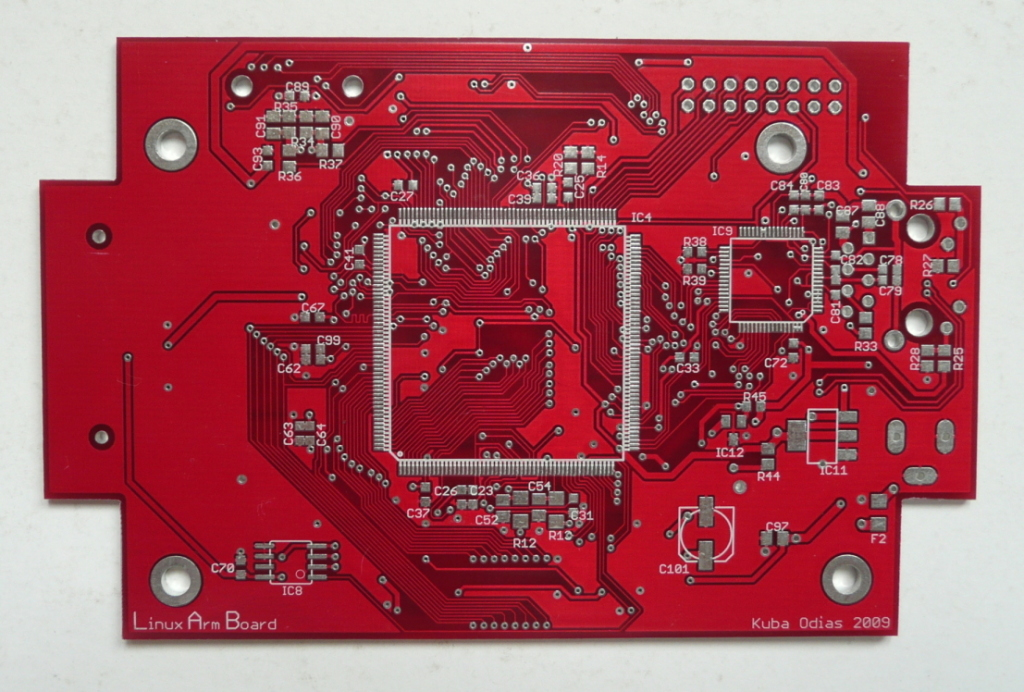
\includegraphics[scale=0.25,angle=90]{img/pcb1_bottom.jpg}}\\
%				\vspace{20pt}
%				\subfigure[Górna strona z przylutowanymi elementami]{\label{fig:pcb1-top}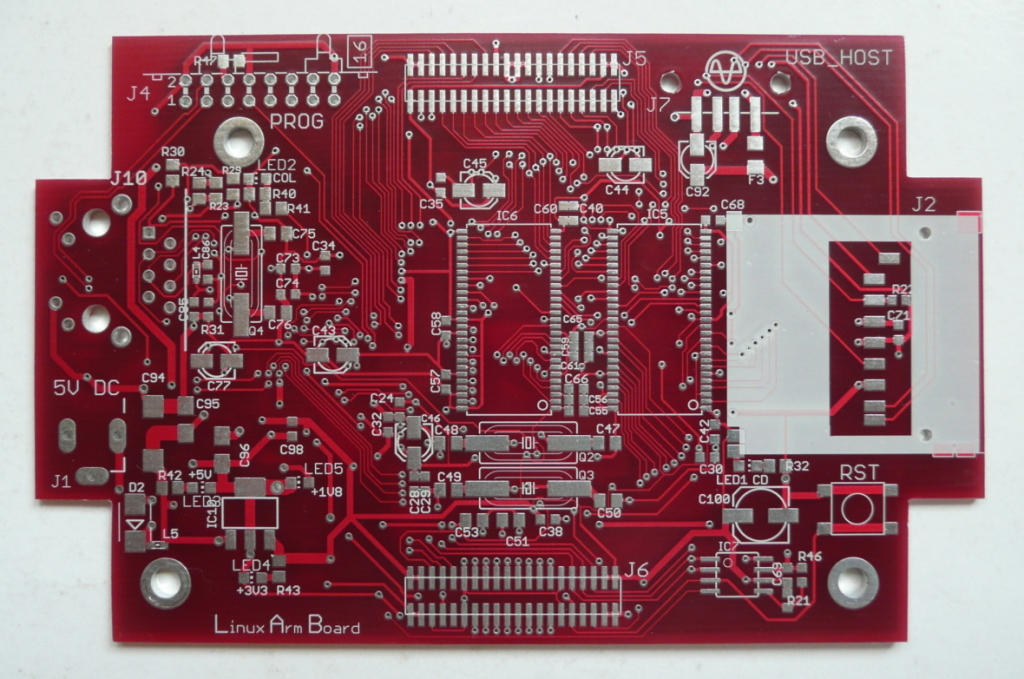
\includegraphics[scale=0.25,angle=90]{img/pcb1_top.jpg}}
%				\hspace{20pt}
%				\subfigure[Dolna strona z przylutowanymi elementami]{\label{fig:pcb1-bottom}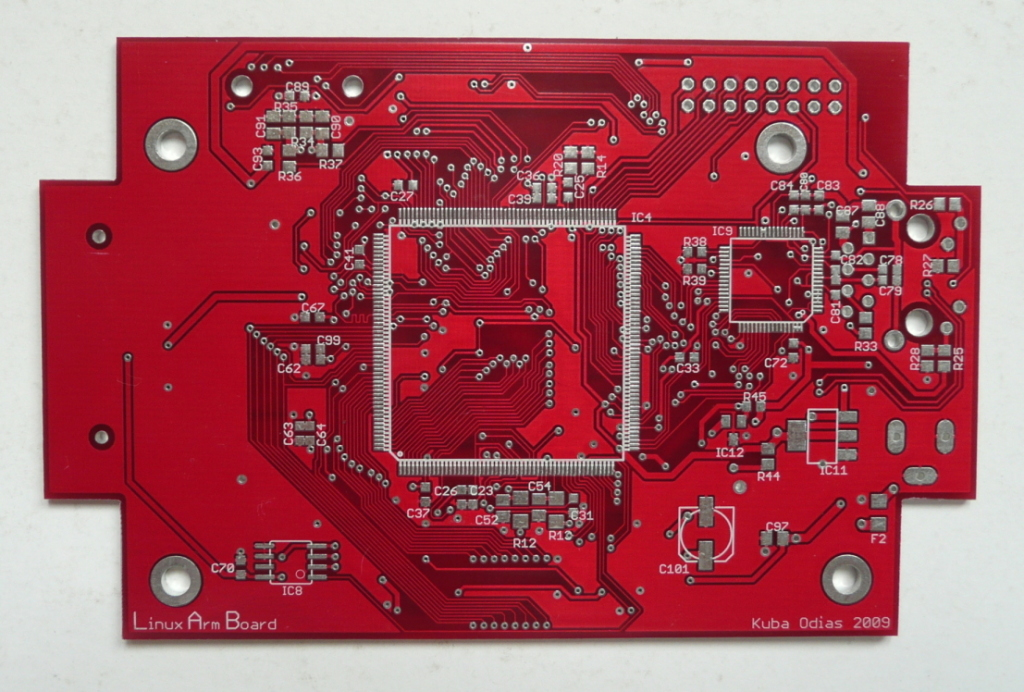
\includegraphics[scale=0.25,angle=90]{img/pcb1_bottom.jpg}}
%			\end{center}
%			\caption{Główna płytka drukowana}
%			\label{fig:pcb1}
%		\end{figure}
%		\begin{figure}[]
%			\begin{center}
%				\subfigure[Górna strona]{\label{fig:pcb2-top}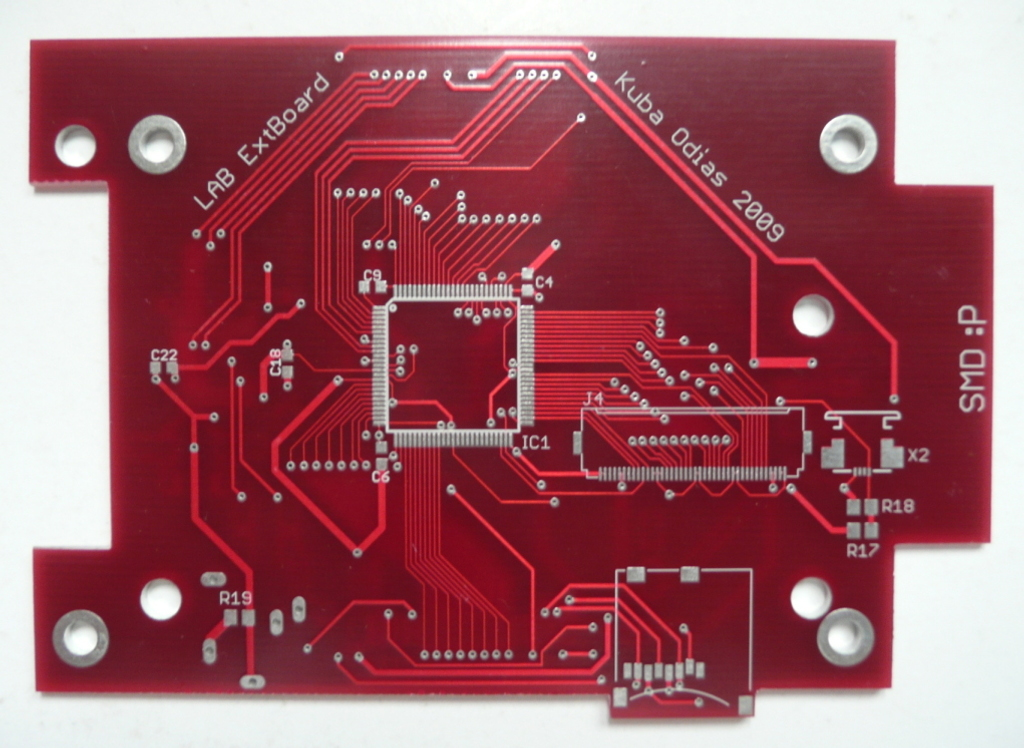
\includegraphics[scale=0.25,angle=90]{img/pcb2_top.jpg}}
%				\hspace{20pt}
%				\subfigure[Dolna strona]{\label{fig:pcb2-bottom}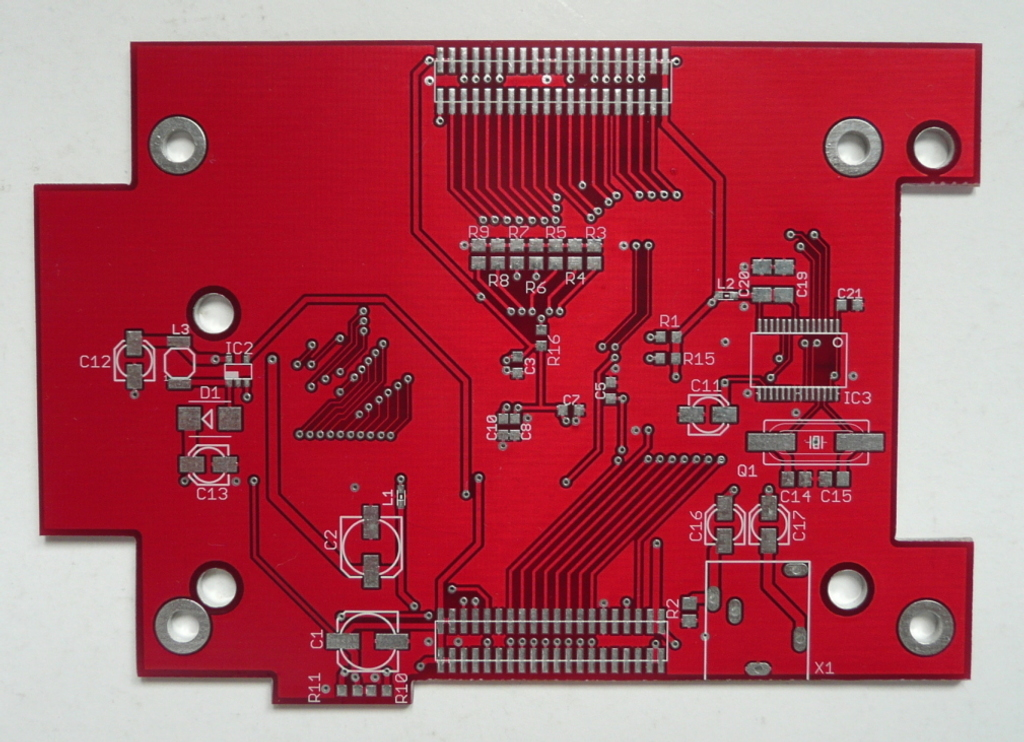
\includegraphics[scale=0.25,angle=90]{img/pcb2_bottom.jpg}}\\
%				\vspace{20pt}
%				\subfigure[Górna strona z przylutowanymi elementami]{\label{fig:pcb2-top}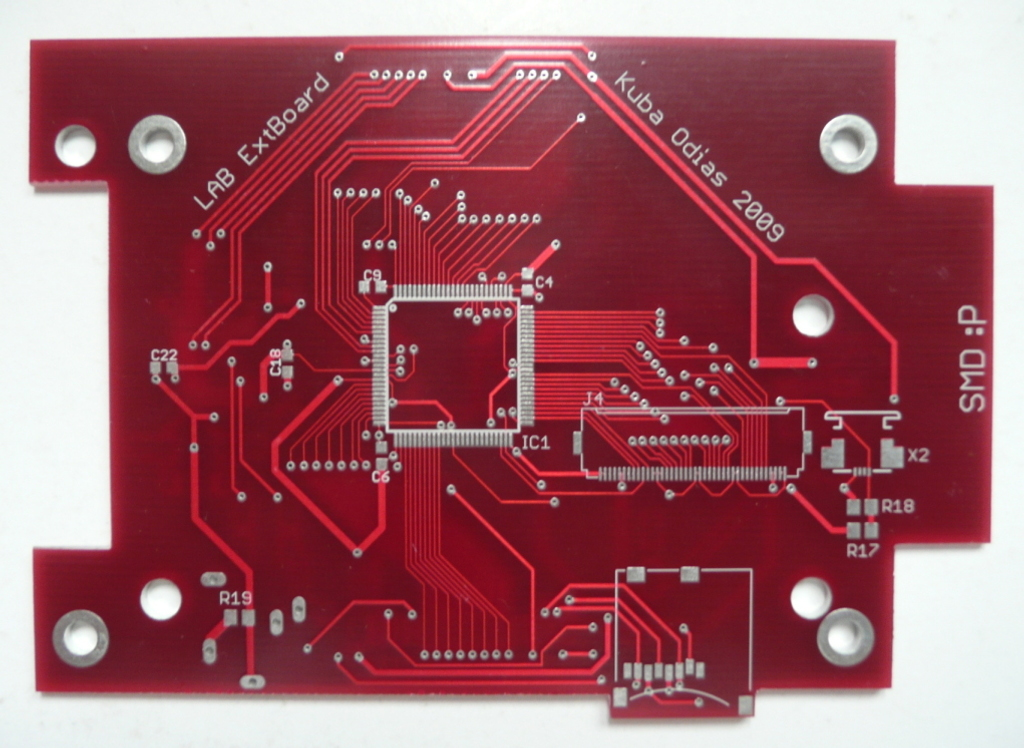
\includegraphics[scale=0.25,angle=90]{img/pcb2_top.jpg}}
%				\hspace{20pt}
%				\subfigure[Dolna strona z przylutowanymi elementami]{\label{fig:pcb2-bottom}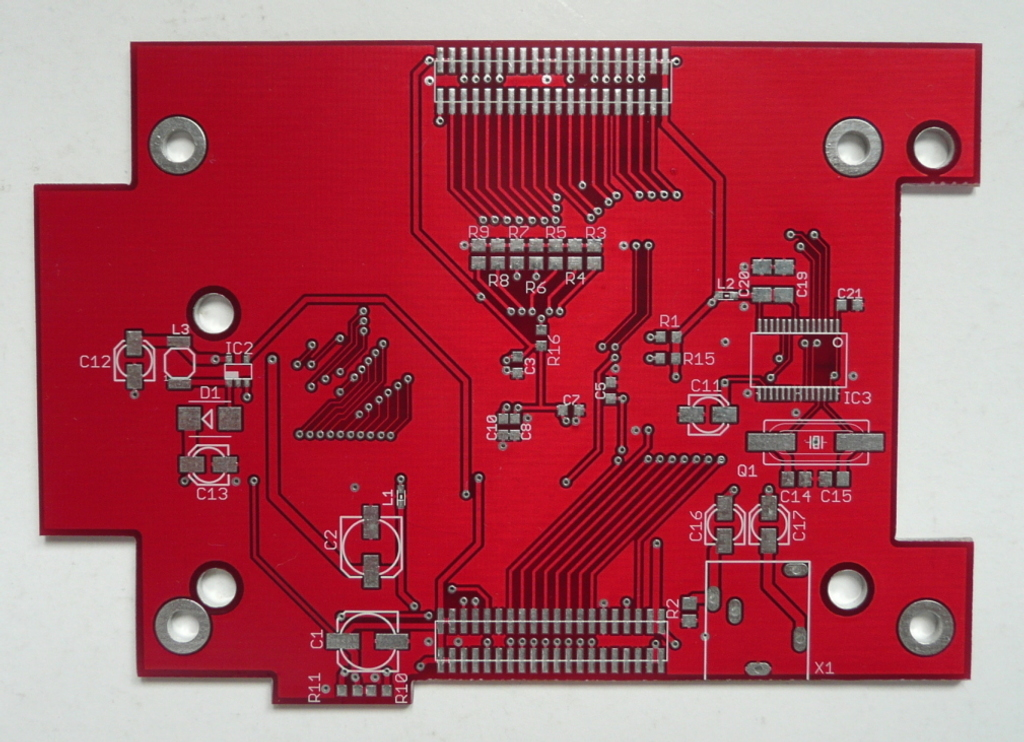
\includegraphics[scale=0.25,angle=90]{img/pcb2_bottom.jpg}}
%			\end{center}
%			\caption{Dodatkowa płytka drukowana}
%			\label{fig:pcb2}
%		\end{figure}
	
	
	\chapter{Przykładowe projekty}
	\label{app:przykladowe_projekty}
	\begin{itemize}
		\item \texttt{http://www.atmel.com/dyn/resources/prod\_documents/doc6103.pdf}\\
			Zestaw uruchomieniowy firmy Atmel dla AT91RM9200.\\
			\scriptsize{(strona sprawdzana 15.08.2009)}
			\normalsize
		\item \texttt{http://blackmesaeast.com.pl/projects/electronics/sarge-single-\\board-computer/}\\
			Projekt autorstwa Grzegorza Rajtara wykorzystujący mikrokontroler AT91RM9200 i kontroler sieciowy STE100P.\\
			\scriptsize{(strona sprawdzana 15.08.2009)}
			\normalsize
		\item \texttt{http://bryndza.boff.pl/index.php?dz=proj\&id=armputer210}\\
			Projekt autorstwa Lucjana Bryndzy pełniący rolę serwera sieciowego.\\
			\scriptsize{(strona sprawdzana 15.08.2009)}
			\normalsize
		\item \texttt{http://www.olimex.com/dev/sam9-L9261.html}\\
			Zestaw uruchomieniowy firmy Olimex dla mikroprocesora AT91SAM9261.\\
			\scriptsize{(strona sprawdzana 15.08.2009)}
			\normalsize
	\end{itemize}
	
\end{document}